\documentclass{article}

% packages
\usepackage{graphicx}
\usepackage{lastpage}
\usepackage{fancyhdr}
\usepackage[hidelinks]{hyperref}
\usepackage{color}
\usepackage{float}

% page margins
\addtolength{\topmargin}{-0.75in}
\addtolength{\oddsidemargin}{-1.0in}
\addtolength{\evensidemargin}{-1.0in}
\addtolength{\textwidth}{2.0in}
\addtolength{\textheight}{1.5in}

% header and footer
\pagestyle{fancy}
\fancyhf{}
\lhead{Fault-Tolerant Quadcopter}
\rhead{\textit{Vaughn, Mayank, Cooper}}
\cfoot{\thepage\ of \pageref{LastPage}}
\rfoot{\today}

% custom commands
\newcommand{\HREF}[2]{{\color{blue}\underline{\smash{\href{#1}{#2}}}}}

% metadata
\title{ECE 453 Project Proposal}
\author{Vaughn Kottler}
\author{Mayank Katwal}
\author{Cooper Green}

\begin{document}

\begin{center}

	{\huge\textbf{ECE 453 Project Proposal} (Fall 2018)}

	{\large University of Wisconsin-Madison}

	{\large\textit{Vaughn Kottler, Mayank Katwal, Cooper Green}}

\end{center}

\section{Introduction}

We are interested in building a \textit{quadcopter} plus
\textit{ground station} and \textit{web-based user interface}.
We have chosen to call this project the
\textbf{fault-tolerant quadcopter}. This name reveals one of our
design goals that will be covered in a future section.

This document serves as the formal proposal to be vetted by the
course instructor,
\HREF{https://directory.engr.wisc.edu/ece/Faculty/Krachey_Joe/}{Joe Krachey}.
We have
\HREF{https://fault-tolerant-quadcopter.readthedocs.io/en/latest/}
{additional documentation in work online} that we plan to keep in
sync with our project's scope and current progress. At the time
of writing it is not yet in a stable state.

This project is designed for three major bodies of work that were
mentioned above but are better captured by \textbf{Figure \ref{fig:high-level}}:

\begin{figure}[H]
	\centering
	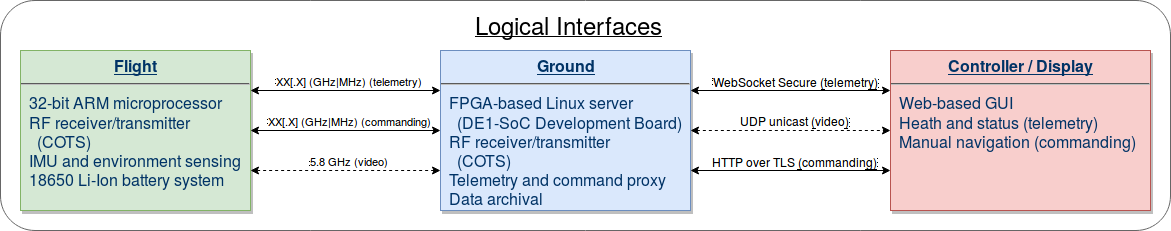
\includegraphics[width=\linewidth]{../src/im/top_level}
	\caption{High-level overview of the major components and
		their interfaces}
	\label{fig:high-level}
\end{figure}

This high-level architecture is inspired by existing aerospace
avionics and software systems that we have done research on
and have some first-hand experience with. Our current, collective
experience with such systems (and the technical challenges we
anticipate being associated with them) is minimal, though. For
this reason \textbf{we seek feedback on our lower-level goals and
approach}, provided that this high-level idea suffices as
a project worth pursuing.

\section{Technical Features}

A vehicle that is \textit{single-fault tolerant} is capable of continuing
nominal operation after experiencing any arbitrary failure in a well-defined
\textit{fault space}. We aim to implement single-fault tolerance by:

\begin{enumerate}
	\item Limiting the initial fault space to a ``loss of ground station
		heartbeat'' event
	\item Executing a ``landing maneuver'' upon fault detection
	\item Iteratively hardening our design to a broader fault space,
		time permitting
\end{enumerate}

We recognize some intermediate milestones that will need to be reached before
an ``automatic flight-termination system'' described above can be expected to
function:

\begin{itemize}
	\item Establish wireless communication between the vehicle and
		ground station
	\item Establish percentage-based throttle control over each motor
	\item Establish manual-commanding capability to the vehicle from a
		web-based user interface
	\item View live telemetry from a web-based user interface
	\item Sense angular velocity via gyroscope and force experienced via
		inertial measurement unit
	\item Develop a control algorithm to fly in a stable hover or
		holding pattern
	\item Extend control algorithm to control for velocity in three axes
		to achieve controlled motion
	\item Sense relative altitude
	\item Extend control algorithm to control for a specific \textit{delta-y}
		(perpendicular to ground plane) 
\end{itemize}

Our limited understanding of control theory and lack of experience in general
with avionics systems may limit what we can achieve in the end, but we
recognize this and have focused on primarily \textit{system-level} goals and
requirements versus specific technical requirements (battery life, thrust and
payload capability, etc.).

\subsection{Quadcopter}

We intend to pursue an implmentation depicted in
\textbf{Figure \ref{fig:quadcopter}}:

\begin{figure}[H]
	\centering
	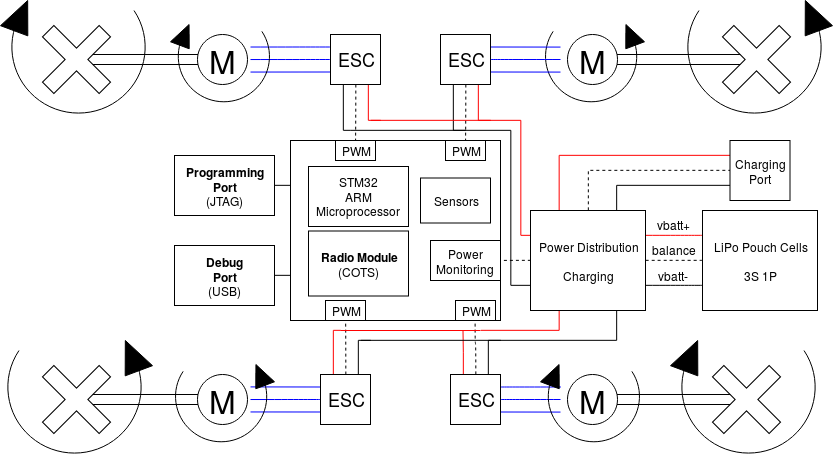
\includegraphics[width=\linewidth]{../src/im/quadcopter}
	\caption{Block diagram view of the quadcopter}
	\label{fig:quadcopter}
\end{figure}

{\large Responsible Engineer: \textbf{Vaughn}}

\pagebreak

\subsection{Ground Station}

We intend to pursue an implmentation depicted in
\textbf{Figure \ref{fig:ground_station}}:

\begin{figure}[H]
	\centering
	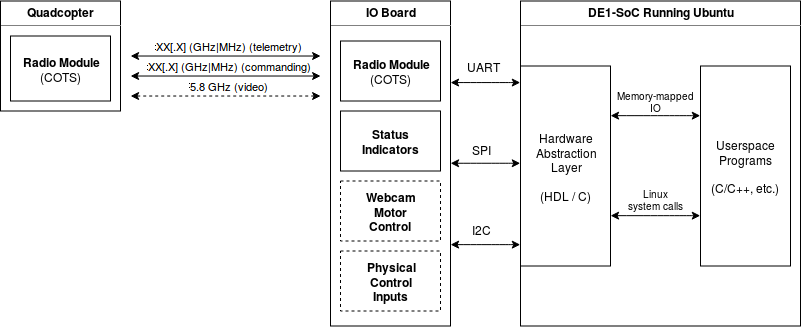
\includegraphics[width=\linewidth]{../src/im/ground_station}
	\caption{Block diagram view of the ground station}
	\label{fig:ground_station}
\end{figure}

{\large Responsible Engineer: \textbf{Cooper}}

\pagebreak

\subsection{Display and Controller}

We intend to pursue an implmentation depicted in
\textbf{Figure \ref{fig:display_controller}}:

\begin{figure}[H]
	\centering
	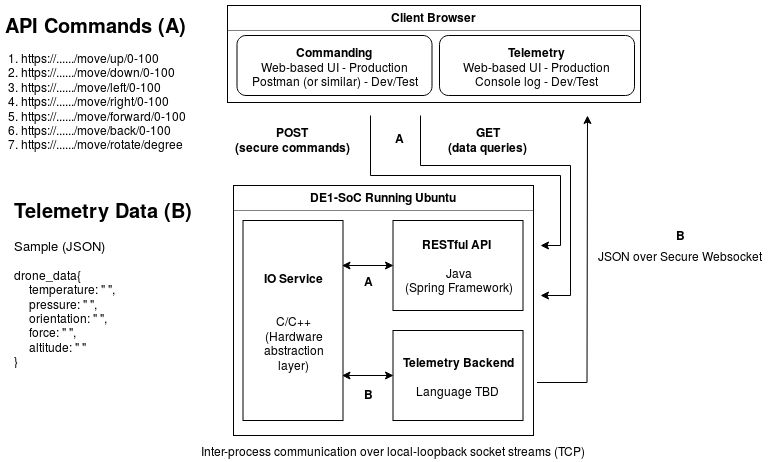
\includegraphics[width=\linewidth]{../src/im/display_controller}
	\caption{Block diagram view of the display and control user
		interface}
	\label{fig:display_controller}
\end{figure}

{\large Responsible Engineer: \textbf{Mayank}}

\section{Roles and Responsibilities}

How we plan to share responsibility.

\subsection{Vaughn Kottler}

\textbf{Responsible Engineer} for the following:

\begin{description}
	\item [Flight Vehicle] TODO
	\item [Control Algorithms] TODO
\end{description}

\subsection{Mayank Katwal}

\textbf{Responsible Engineer} for the following:

\begin{description}
	\item [Telemetry Display] TODO
	\item [Vehicle Controller] Hardware of Software
\end{description}

\subsection{Cooper Green}

\textbf{Responsible Engineer} for the following:

\begin{description}
	\item [Ground Station] TODO
	\item [Radio Frequency Communication] TODO
\end{description}

\section{Project Management}

\begin{quote}
	\textit{``If I had an hour to solve a problem I'd spend 55 minutes
	thinking about the problem and 5 minutes thinking about
	solutions.'' - Albert Einstein}
\end{quote}

TODO

\subsection{Initial Development and Prototyping}

TODO

\subsection{Final Stages}

TODO

\end{document}
